\documentclass{article}
\usepackage{graphicx}
\usepackage{caption}
\usepackage[margin=1in]{geometry}
\begin{document}

\begin{figure}[ht]
\centering
\begin{minipage}{0.48\textwidth}
\centering
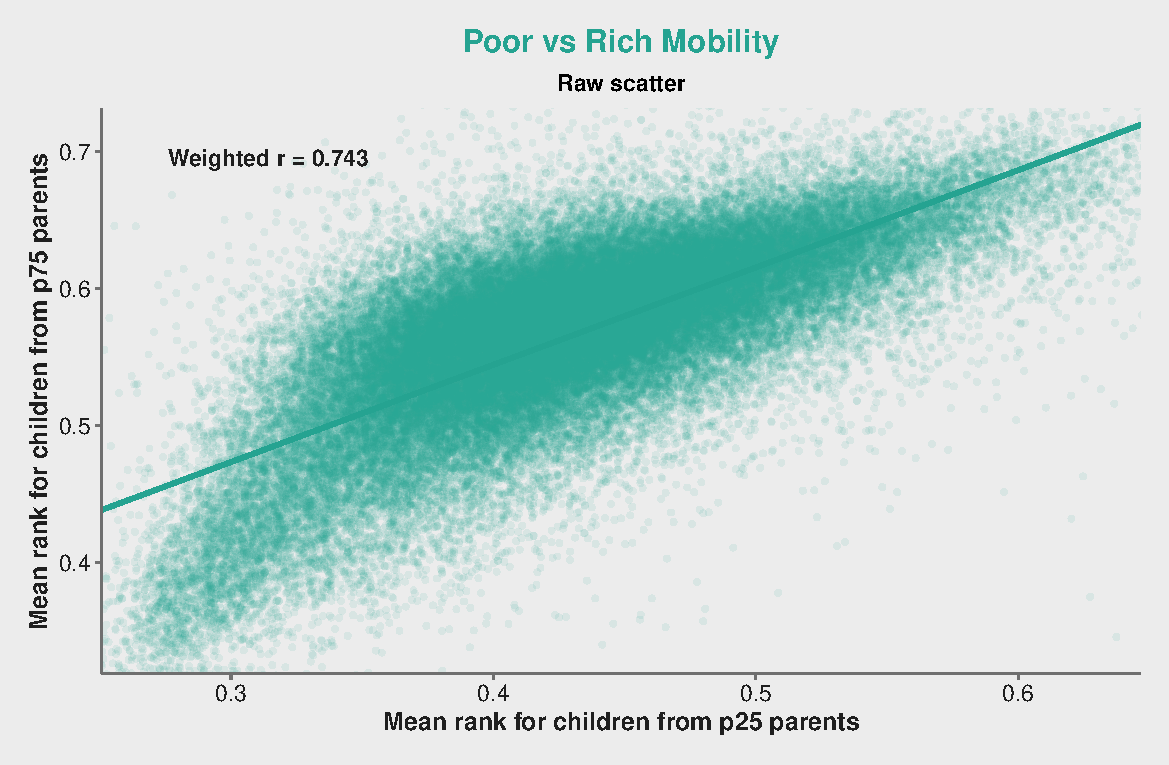
\includegraphics[width=\linewidth]{../figures/poor_rich_raw_R.pdf}
\caption*{A. Raw scatter}
\end{minipage}\hfill
\begin{minipage}{0.48\textwidth}
\centering
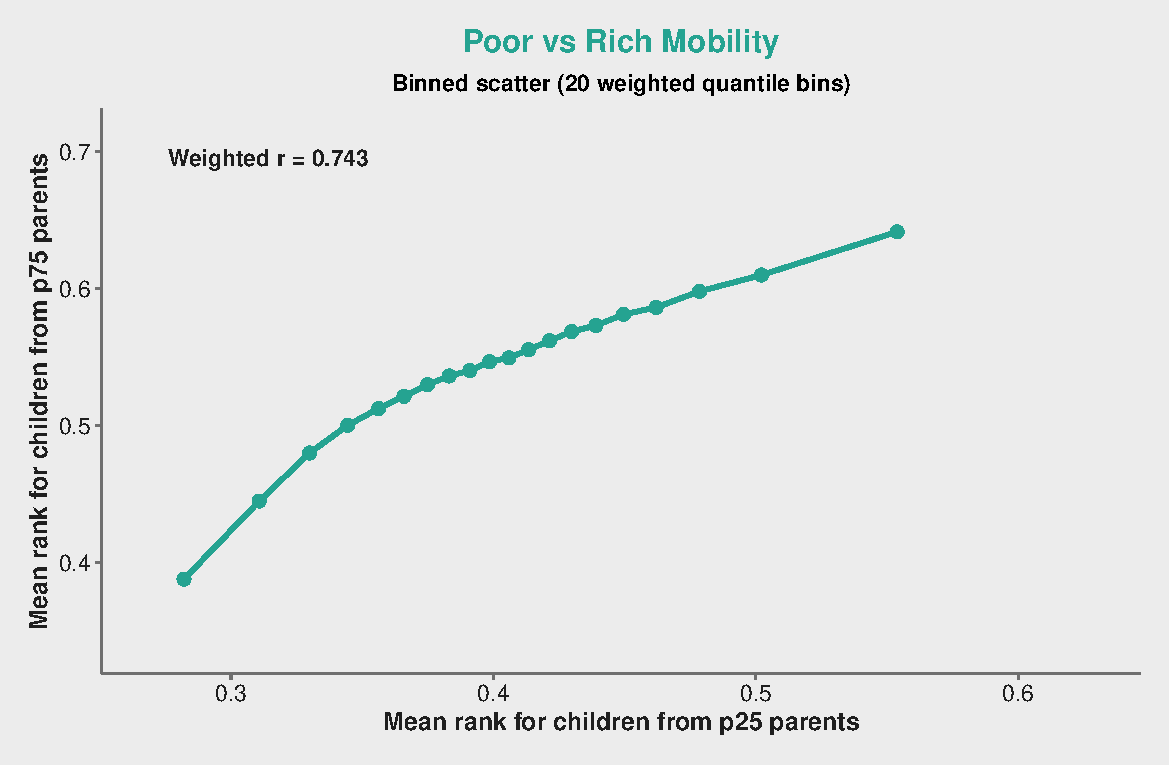
\includegraphics[width=\linewidth]{../figures/poor_rich_bins_R.pdf}
\caption*{B. Binned scatter}
\end{minipage}
\caption{Tract-level mobility (p25 vs p75). Weighted r values: raw 0.743, binned 0.743.}
\end{figure}

\begin{figure}[ht]
\centering
\begin{minipage}{0.48\textwidth}
\centering
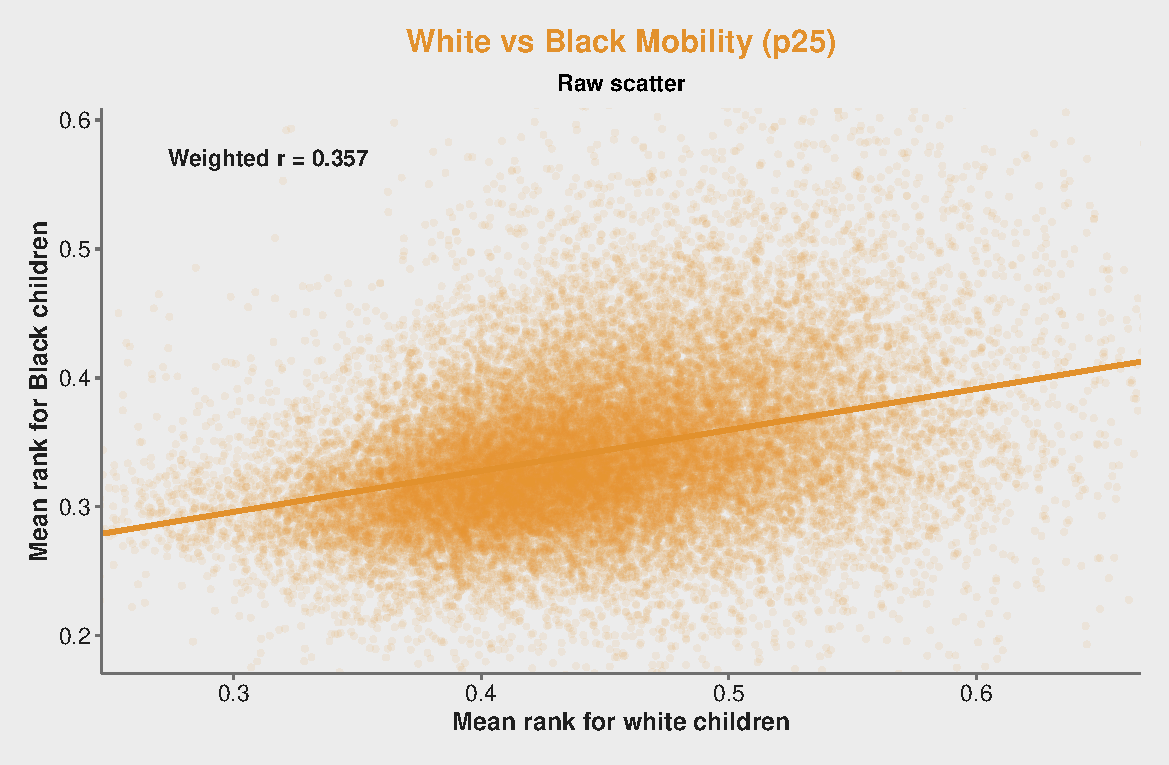
\includegraphics[width=\linewidth]{../figures/white_black_raw_R.pdf}
\caption*{A. Raw scatter}
\end{minipage}\hfill
\begin{minipage}{0.48\textwidth}
\centering
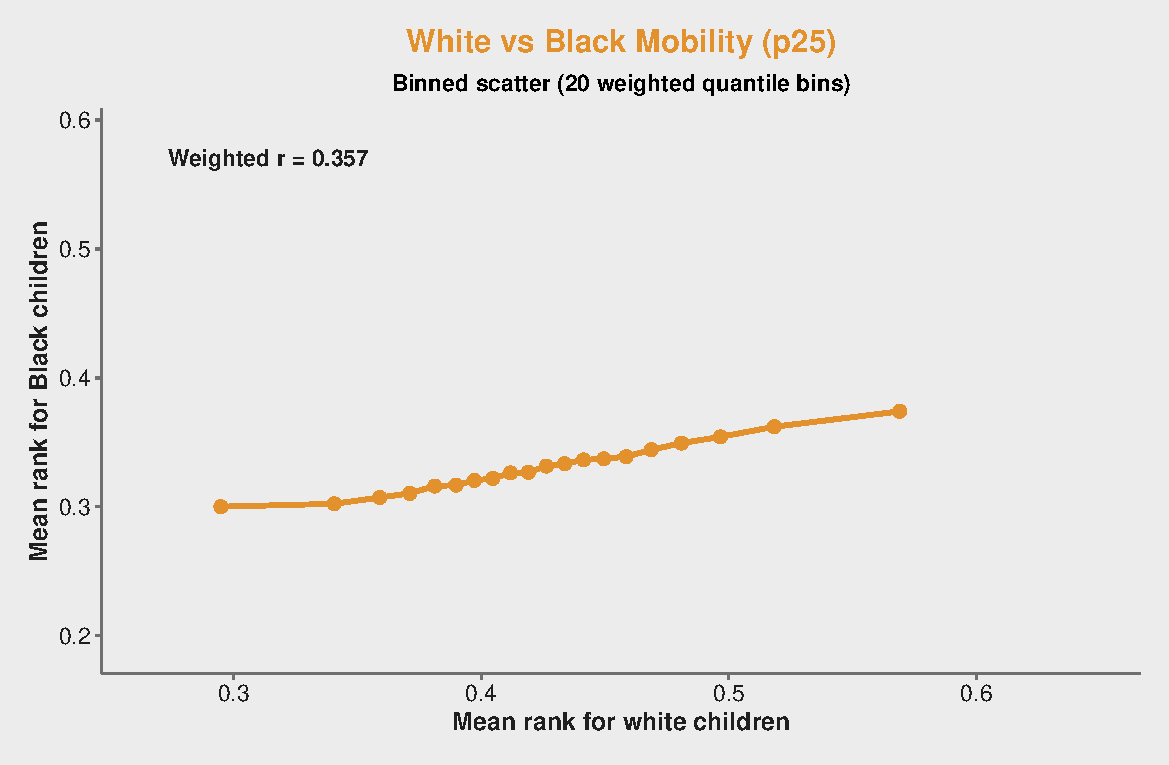
\includegraphics[width=\linewidth]{../figures/white_black_bins_R.pdf}
\caption*{B. Binned scatter}
\end{minipage}
\caption{Tract-level mobility (white vs Black, p25). Weighted r values: raw 0.357, binned 0.357.}
\end{figure}

\end{document}
